\title{LIGHTNING ORDER restaurant management application}
\documentclass[oneside,12pt]{book}  
\usepackage[italian]{babel}
\usepackage[utf8x]{inputenc}
\usepackage{array,multirow}
\usepackage{longtable}
\usepackage{listings}
\usepackage{ragged2e}
\usepackage{color}
\usepackage{setspace}
\usepackage{amsmath}
\usepackage{geometry,color,graphicx,float}
\usepackage[colorinlistoftodos]{todonotes}
\usepackage{glossaries}
\usepackage{xcolor,colortbl}
\definecolor{Red}{rgb}{1,0,0}
\definecolor{Blue}{rgb}{0.8,0.5,1}
\definecolor{Green}{rgb}{0.5,1,0.5}
\definecolor{LightCyan}{rgb}{0.88,1,1}

\usepackage{booktabs}% http://ctan.org/pkg/booktabs
\newcommand{\tabitem}{{\textbullet}~}
\usepackage{pdfpages}

\usepackage{fancyhdr}

\pagestyle{fancy}
\fancyhf{}
\cfoot{\thepage}
\rhead{\textsc{\chaptername \space \thechapter} }

\begin{document}

\begin{titlepage}

\newcommand{\HRule}{\rule{\linewidth}{0.3mm}}
\center


\includegraphics[width=50mm]{logo_unina.png}\\
\vfill
\textsc{\LARGE \bfseries Università degli Studi di Napoli "Federico II"}\\[0.7cm] % Name of your university/college
\textsc{\large \bfseries Scuola Politecnica e delle Scienze di Base}\\
\textsc{\large \bfseries Corso di Laurea Magistrale in Ingegneria Informatica}\\
\vfill
\textsc{\large Elaborato Software Architecture Design} \\[0.6cm]
\textbf{\Large LIGHTNING ORDER}\\[0.2cm]
\textsc{\large Restaurant management application}\\
\vfill
%\large \textbf{Subject code} \\[0.2cm]
\bfseries{\large
Antonio Emmanuele - M6300\\
Giuseppe Francesco Di Cecio - M63001211\\
Giuseppe De Rosa - 00119123\\
Nicola D'Ambra - M63001223\\[0.5cm]
}

\vfill
{\text \large A.A. 2020/2021}
\end{titlepage}

\thispagestyle{empty}
\tableofcontents
\pagenumbering{arabic}
\chapter{Introduzione}
\chapter{Processo di sviluppo}
Il processo di sviluppo utilizzato per la realizzazione del software è \textbf{UP} (Unified Process). Un processo di tipo agile ci ha permesso quindi in brevi tempi di avere un'implementazione funzionante del software, anche se non soddisfa tutti i casi d'uso richiesti.
\\Data la grande dimensione dell'applicazione e i tempi ridotti di consegna, l'utilizzo di un processo \textit{guidato da piani} avrebbe generato non pochi problemi.

\section{Github}
In un primo approccio alla realizzazione del sistema si è deciso di utilizzare \textbf{Github} come piattaforma di condivisione di codice, modello e documentazione. Fin dall'inizio il lavoro è stato diviso in tre repository indipendenti:
\begin{itemize}
	\item Una repository che contiene tutti i file di documentazione e di modellazione del software.
	\item Una repository che contiene solo la parte di software \textit{backend}. 
	\item Una repository che contiene solo la parte di software \textit{frontend}.
\end{itemize}
Il motivo della divisione del codice in più repository è quello di scollegare fisicamente la realizzazione delle due parti. Inoltre il \textit{frontend} è pensato per essere implementato su una piattaforma Android, mentre il \textit{backend} su una piattaforma Desktop, accentuando tale suddivisione.
\\In ogni repository sono state create delle \textit{Branch} per permettere uno sviluppo parallelo tra i vari componenti del gruppo. Infatti durante la realizzazione ogni componente si è occupato di un lavoro, al termine dei quali si poteva continuare con un \textit{Merge} per unirli.

\section{UP}
Il processo di sviluppo software UP prevede lo sviluppo in iterazioni. Ognuna delle quali comprende \textit{analisi}, \textit{progettazione}, \textit{implementazione} e \textit{test}.
\\Prima di tutto si è effettuata una fase di \textbf{ideazione}, per poi proseguire con la fase di \textbf{elaborazione} (che comprende le iterazioni vere e proprie) ed infine una fase di \textbf{transazione} per rilasciare una piccola versione ed illustrarne il funzionamento.

\subsection{Ideazione}
Nei primi giorni si è deciso \textit{cosa} il sistema dovesse fare. In particolare sono stati identificati gli attori che avrebbero preso parte all'applicativo e per ogni attore gli obiettivi da raggiungere. Sono stati valutati i requisiti considerando anche il tempo che si aveva a disposizione per non sfociare in un progetto troppo complesso da realizzare.
\\In seguito si è effettuato uno studio di fattibilità, volto a capire se il sistema poteva essere realizzato con gli strumenti che si avevano a disposizione. 
\\Nel dettaglio nella fase di ideazione sono state eseguite le seguenti azioni:
\begin{itemize}
	\item Workshop dei requisiti, attraverso il confronto con gli stackholder (alcuni componenti del gruppo hanno lavorato e/o lavorano ancora nell'ambito della ristorazione).
	\item Identificazione degli attori.
	\item Descrizione breve dei primi casi d'uso ricercati.
	\item Descrizione dettagliata dei casi d'uso più importanti, quelli che rappresentavano il "cuore" del sistema e che racchiudevano le funzionalità di principale interesse.
	\item Architettura di alto livello 	
\end{itemize} 

\subsection{Elaborazione}
La fase di elaborazione è stata divisa in tre iterazioni di all'incirca 1-2 settimane ciascuna.
\begin{enumerate}
	\item Nella prima iterazione sono stati analizzati i requisti più nello specifico focalizzando l'attenzione sulla logica centrale del sistema, costruendo:
	\begin{itemize}
		\item Analisi
		\begin{itemize}
			\item Modello di dominio
			\item Sequence Diagram di sistema
			\item Comunicazione tra Business Logic e Database
		\end{itemize}
		\item Progetto
		\begin{itemize}
			\item Progetto dell'architettura del sistema
			\item Progetto della base di dati
			\item Progetto dell'architettura del Main System
			\item Class Diagram di dettaglio della Business Logic
			\item Sequence Diagram di dettaglio
		\end{itemize}
		\item Implementazione
		\begin{itemize}
			\item Implementazione Business Logic (BL)
			\item Implementazione del database (DB)
		\end{itemize}
		\item Test
		\begin{itemize}
			\item Test di unità della BL
			\item Test di unità del database
			\item Test di integrazione tra BL e DB
		\end{itemize}
	\end{itemize}

	\item Nella seconda iterazione:
	\begin{itemize}
		\item Analisi
		\begin{itemize}
			\item Comunicazione tra Business Logic, Broker e Request Generator
			\item Comunicazione tra Proxy e Main System
		\end{itemize}
		\item Progetto
		\begin{itemize}
			\item Class diagram di dettaglio del Broker
			\item Class diagram di dettaglio del Request Generator
			\item Class diagram di dettaglio dei Proxy
		\end{itemize}
		\item Implementazione
		\begin{itemize}
			\item Implementazione del Broker
			\item Implementazione del Request Generator
			\item Implementazione dei Proxy
		\end{itemize}
		\item Test
		\begin{itemize}
			\item Test di unità del Broker
			\item Test di unità del Request Generator
			\item Test di unità del Proxy
		\end{itemize}
	\end{itemize}
	\item Nella terza iterazione ci si è focalizzati sul lato \textit{frontend} per rilasciare un applicativo accessibile dall'utente.
		\begin{itemize}
			\item Analisi
			\begin{itemize}
				\item Comunicazione tra Proxy e Applicazione Android
				\item Formato dei messaggi da scambiare
			\end{itemize}
			\item Progetto
			\begin{itemize}
				\item Progetto dell'architettura Android
			\end{itemize}
			\item Implementazione
			\begin{itemize}
				\item Implementazione dell'architettura 
			\end{itemize}
			\item Test
			\begin{itemize}
				\item Test di comunicazione tra Android e Sistema
			\end{itemize}
		\end{itemize}
\end{enumerate}

\subsection{Transazione}
Teoricamente il sistema prevede tre tipi di applicazioni:
\begin{itemize}
	\item Una per dispositivi mobile Android
	\item Una per il sistema centrale, installabile su un sistema con un interprete Java e un database PostgreSQL
	\item Una per dispositivi Desktop 
\end{itemize}
Per motivi di tempistiche si è scelto di implementare solo le prime due. Per tutti i dipendenti un'applicazione Android, la quale viene rilasciata in formato \textit{.apk} con compatibilità minima del sistema operativo \textit{Lollipop 5.0}.

\chapter{Documento di visione}
\chapter{Specifica dei Requisiti}
Per avere una visione chiara di ciò che si deve costruire, quindi una descrizione dettagliata dei requisiti, sono stati effettuati dei colloqui con degli stakeholders e delle sessioni di "brainstorming" tra i componenti del gruppo. In seguito si è costruito un diagramma dei casi d'uso i quali sono stati poi descritti dettagliatamente.
\\Prima di elencare e descrivere i casi d'uso, è necessario identificare gli attori che caratterizzeranno il sistema.

\section{Attori Primari}
\begin{figure}[H]
	\centering
	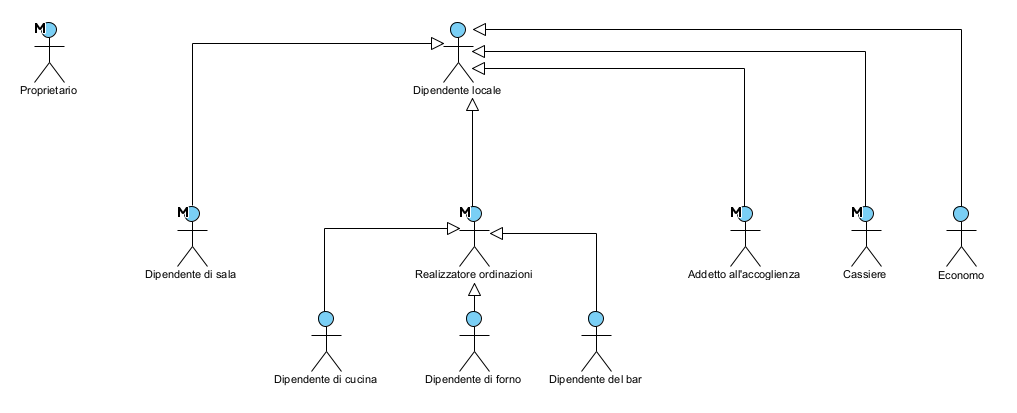
\includegraphics[width=\textwidth]{Immagini/AttoriPrimari.png}
\end{figure}

\begin{itemize}
	\item Dipendente di sala: deve interagire con il cliente e prendere le ordinazioni in maniera tale che vengano smistate, tramite il sistema alle varie attività del locale;
	\item Dipendenti di cucina/forno/bar: usano il sistema per ricevere i vari ordini e per notificare un completamento di essi;
	\item Addetto all'accoglienza: usa il sistema per visualizzare i tavoli disponibili ed assegnarli ai clienti;
	\item Cassiere: richiede al sistema il conto totale di un cliente interessato per completare il pagamento;
	\item Economo: si occupa della gestione delle merci ovvero l'aggiornamento delle quantità presenti in magazzino (in base alle vendite effettuate dalla sala e dalle richieste dei realizzatori di ordinazioni);
	\item Proprietario: può usare il sistema per aggiungere e rimuovere dipendenti, consultare dati come vendite, guadagni, quantità di merci.
\end{itemize}
Nella realtà non tutti gli attori descritti corrisponderanno a persone fisiche differenti, infatti alcuni dipendenti potranno assumere le funzionalità di più attori (ad esempio un dipendente di sala potrebbe ricoprire anche il ruolo di addetto all'accoglienza). A tal proposito quindi si è scelto di intendere gli attori come \textbf{ruoli} che un dipendente reale possa ricoprire.

\section{Attori Finali}
\begin{figure}[H]
	\centering
	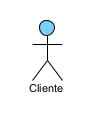
\includegraphics[width=0.12\textwidth]{Immagini/AttoriFinali.png}
\end{figure}

\begin{itemize}
	\item Cliente: pur non interagendo con il sistema, è direttamente interessato in alcuni suoi casi d'uso in quanto gli consentono di usufruire del servizio del locale
\end{itemize}
\newpage

\section{Tabella Attori-Obiettivi}
Dopo aver identificato a pieno gli attori che utilizzeranno il sistema, bisogna associare ad ogni attore i suoi obiettivi.
\begin{table}[!h]
	\centering
	\begin{tabular}{|p{0.3\linewidth}|p{0.65\linewidth}|}
		\hline
		\rowcolor{Red}
		Attore & Obiettivi \\
		\hline
		\hline
		\multirow{9}{6em} {Proprietario} & Inserimento di un dipendente \\
		& Rimozione di un dipendente \\ & Modifica dei ruolo di un dipendente \\
		& Visualizzazione dei dipendenti \\
		& Inserimento di un tavolo\\
		& Rimozione di un tavolo\\
		& Modifica di un tavolo\\
		& Visualizzazione dei tavoli \\
		& Inserimento di prodotti nel menu \\
		& Rimozioni di prodotti dal menu \\
		& Modifica di prodotti del menu \\
		& Visualizzazione del menu completo \\
		
		\hline
		\multirow{4}{6em} {Dipendente di sala} 
		& Creazione di un'ordinazione per un cliente  \\
		& Rimozione di un'ordinazione \\ 
		& Modifica di un'ordinazione \\
		& Visualizzazione delle ordinazioni \\
		\hline
	
		\multirow{3}{6em} {Accoglienza} 
		& Assegnazione di un tavolo a dei clienti  \\
		& Modifica dello stato di un tavolo (libero, occupato, riservato, ecc.) \\ 
		& Visualizzazione di tutti i tavoli \\
		\hline	
		
		\multirow{1}{6em} {Cassiere} 
		& Generazione vendita di un tavolo (pagamento dei clienti)\\ 
		\hline
		
		\multirow{2}{7em} {Realizzatore di ordinazione} 
		& Visualizzazione degli ordini per area (cucina, bar, forno)  \\
		& Notifica completamento ordinazione \\ 
		\hline
		
		\multirow{4}{6em} {Economo} 
		& Inserimento di una merce  \\
		& Modifica di una merce \\ 
		& Rimozione di una merce \\
		& Visualizzazione di una merce \\
		\hline
	\end{tabular}
\end{table}
\\Gran parte degli obiettivi riguardano operazioni \textit{CRUD} (Create, Read, Update, Delete) che possono essere raggruppate in un solo obiettivo.

\newpage
\section{Diagramma dei Casi D'Uso}
Tutti gli obbiettivi CRUD dei vari attori sono stati inglobati in un unico caso d'uso con il prefisso \textbf{Gestisci}, per indicare le operazioni che racchiudono.
\\
\\
\begin{centering}  
	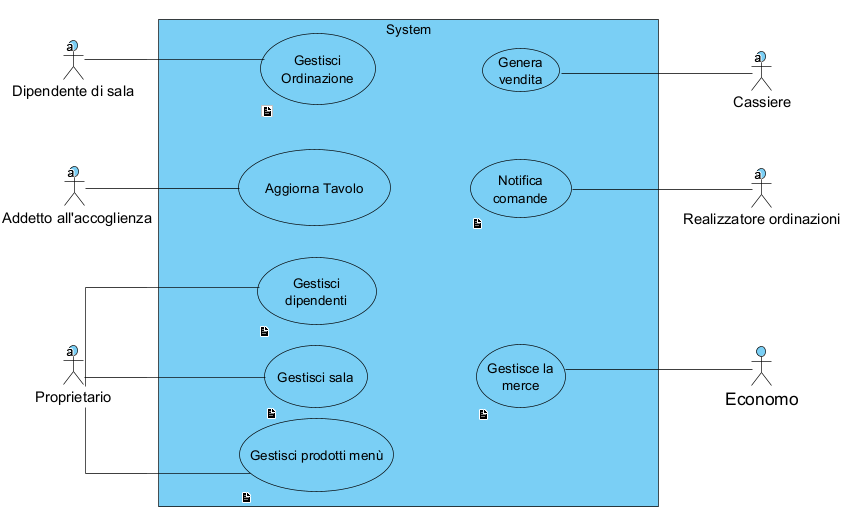
\includegraphics[width=\textwidth]{Immagini/DiagrammaCasiUso.png}
\end{centering}

\subsection{Descrizione Breve}
\subsubsection{Gestisci Ordinazione}
Come descritto in precedenza questo caso d'uso racchiude le operazioni CRUD riguardo ad un'ordinazione di uno o più clienti. Il cameriere infatti deve essere in grado di creare un'ordinazione per un cliente e poterla in seguito modificare, visualizzare o addirittura rimuovere dal sistema.

\subsubsection{Aggiorna Tavolo}
L'addetto all'accoglienza si occupa di far accomodare i clienti nella sala. Il suo obiettivo è quindi avere una visione completa dei tavoli comunicando tramite il sistema  quali tavoli hanno clienti in attesa di ordinazione, quali sono liberi e quali sono occupati.

\subsubsection{Gestisci Dipendenti}
Il proprietario può aggiungere/rimuovere dipendenti dal sistema ed inoltre è in grado di decidere/modificare i ruoli o il ruolo di ogni dipendente durante il servizio.

\subsubsection{Gestisci Sala}
Il proprietario può indicare l'identificativo di ogni tavolo in relazione alla sala in cui appartiene. Gli altri dipendenti quindi posso accedere tramite l'identificativo a tutte le informazioni che riguardano i tavoli (numero di persone accomodate, lista dei prodotti ordinati, ecc).

\subsubsection{Gestisci Prodotti Menù}
Il proprietario può effettuare operazioni CRUD per la gestione del menù del locale.

\subsubsection{Genera Vendita}
Il compito del cassiere è quello di registrare il pagamento dei clienti in relazione a ciò che hanno ordinato. Esso quindi deve poter risalire tramite il tavolo a tutti gli ordini associati ai clienti per ricavare il prezzo complessivo da pagare.

\subsubsection{Notifica Ordinazione}
Per rendere il sistema quanto più automatizzato possibile, i realizzatori di ordinazioni (cuoco, pizzaiolo, etc.) devono notificare il completamento di un'ordinazione tramite il sistema. In questo modo, inviando una notifica il sistema provvederà ad avvisare altri dipendenti in attesa di quel completamento.

\subsubsection{Gestisci Merce}
Ogni prodotto del menu è composto da un insieme di merci disponibili in magazzino. Il compito dell'economo è quindi quello di gestire le merci, per avere sotto controllo le merci in esaurimento. L'esaurimento di una merce comporta la non disponibilità di tutti i prodotti del menu che la contenevano.

\subsection{Descrizione Dettagliata}
La descrizione dettagliata è stata fatta solo per i casi d'uso di rilievo.

\begin{longtable}[htbp]{|p{0.3\linewidth}|p{0.65\linewidth}|}
	\hline
		\rowcolor{Blue}	
	\textbf{Titolo} & Gestisci Ordinazione \\[0.3cm]
	\hline
	\textbf{Livello} & Obiettivo Utente \\[0.3cm]
	\hline
	\textbf{Portata} & Applicazione Android o interfaccia Desktop \\[0.3cm]
	\hline
	\textbf{Attore Primario} & Dipendente di sala \\[0.3cm]
	\hline
	\multirow{8}*{\textbf{Parti Interessate}} 
	& \textendash \underline{Dipendenti di sala} (vogliono eseguire le loro mansioni) \\
	& \textendash \underline{Proprietario} (vuole che i clienti siano soddisfatti dal servizio) \\
	& \textendash \underline{Clienti} (vogliono essere serviti nel miglior modo possibile) \\
	& \textendash \underline{Realizzatore di ordinazioni} (vuole ricevere le ordinazioni) \\[0.3cm]
	\hline
	\multirow{8}*{\textbf{Pre-Condizioni}}
	& \textendash Il dipendente di sala non può gestire ordinazioni dei tavoli non suoi \\
	& \textendash Il dipendente di sala non può aggiungere prodotti ad ordinazioni già completate \\
	& \textendash Il dipendente di sala non può rimuove prodotti in lavorazione di una ordinazione \\
	& \textendash Il dipendente di sala non può rimuovere merce ad un prodotto in lavorazione \\[0.3cm]
	\hline
	\multirow{5}*{\textbf{Garanzia di successo}}
	& \textendash Una ordinazione viene creata/modificata/rimossa \\
	& \textendash Una notifica viene inviata ad un realizzatore di ordinazione \\
	& \textendash La merce numerabile costituente i prodotti viene riservata per l’ordinazione \\[0.3cm]
	\hline
	\multirow{5}*{\textbf{Scenario Principale}} 
	& 1. Dipendente di sala visualizza i tavoli in attesa di ordinazione di una sala \\
	& 2. Dipendente di sala seleziona un tavolo \\\
	& 3. Dipendente di sala visualizza ordinazioni tavolo \\
	& 4. Dipendente di sala visualizza ordinazione\\[0.3cm]
	\hline
	\newpage
	\multirow{28}*{\textbf{Estensioni}}
	& 3.A Dipendente di sala inizia ordinazione a tavolo \\
	& 4.A Cliente comunica i prodotti \\
	& 5.A Il dipendente di sala inserisce prodotti con eventuali merci aggiuntive \\
	& 6.A Il cliente comunica preferenza di consegna per prodotti \\
	& 7.A Il dipendente di sala inserisce la preferenza di consegna \\
	& 8.A Il dipendente di sala aggiunge ordinazione \\
	& 9.A Il sistema viene aggiornato \\
	& 10.A Vengono inviate notifiche in maniera  intelligente ai realizzatori di ordinazioni \\
	& \\
	& 3.B Il dipendente di sala rimuove una ordinazione \\
	& 4.B Il sistema viene aggiornato \\
	& 5.B Viene notificato l’evento ad eventuali realizzatori precedentemente notificati \\
	& \\
	& 4.C Cliente comunica al dipendente di modificare un prodotto all'interno di un'ordinazione \\
	& 5.C Dipendente di sala modifica l'ordinazione con i nuovi prodotti \\
	& 6.C Dipendente di sala inoltra la modifica \\
	& 7.C Il sistema inoltra la modifica ai corrispondenti realizzatori \\
	
	& \\
	& 4.D Cliente comunica al dipendente di aggiungere un prodotto all'interno di un'ordinazione \\
	& 5.D Dipendente aggiunge il prodotto (o i prodotti) all'ordinazione \\
	& 6.D Il sistema viene aggiornato e invia una notifica ai realizzatori \\
	
	& \\
	& 4.E Cliente comunica al dipendente di rimuovere un prodotto all'interno di un'ordinazione \\
	& 5.E Dipendente rimuove il prodotto (o i prodotti) all'ordinazione \\
	& 6.E Il sistema viene aggiornato e invia una notifica ai realizzatori \\[0.3cm]
	
	\hline
	\multirow{10}*{\textbf{Scenari Alternativi}}
	& 4.A.1 Prodotto comunicato non è disponibile \\
	& 4.A.2 Ripeti 4.A \\
	& \\
	& 3.B.1 Ordinazione non rimovibile (già completata) \\
	& 3.B.2 Ripeti 3.B \\
	& 4.C.1 L'ordinazione non è modificabile (poichè in lavorazione) \\
	& 4.C.2 Ripeti 4.C \\
	& \\
	& 4.D.1 Il prodotto non è disponibile \\
	& 4.D.2 Ripeti 4.D \\
	& \\
	& 4.E.1 Il prodotto non è rimovibile (poichè in lavorazione) \\
	& 4.E.2 Ripeti 4.E \\[0.3cm]
	\hline
\end{longtable}
\vfill
\begin{longtable}[htbp]{|p{0.3\linewidth}|p{0.65\linewidth}|}
	\hline
	\rowcolor{Green}
	\textbf{Titolo} & Notifica Ordinazione \\[0.3cm]
	\hline
	\textbf{Livello} & Obiettivo Utente \\[0.3cm]
	\hline
	\textbf{Portata} & Applicazione Android o interfaccia Desktop \\[0.3cm]
	\hline
	\textbf{Attore Primario} & Realizzatore di ordinazione \\[0.3cm]
	\hline
	\multirow{8}*{\textbf{Parti Interessate}} 
	& \textendash \underline{Realizzatore di ordinazione} (vuole notificare l’aver completato uno o più lavori, altri realizzatori inoltre possono aspettare questa notifica come segnale per poter iniziare il loro lavoro). \\
	& \textendash \underline{Cliente} (vuole ricevere l’ordinazione). \\
	& \textendash \underline{Proprietario} (vuole che cliente riceva l’ordinazione) \\[0.3cm]
	\hline
	\multirow{1}*{\textbf{Pre-Condizioni}}
	& \textendash L'ordinazione da notificare esiste \\[0.3cm]
	\hline
	\newpage
	\multirow{6}*{\textbf{Garanzia di successo}}
	& \textendash Prodotto in ordinazione viene posto in stato di terminato \\
	& \textendash Qualora i prodotti di tutta l’ordinazione vengano posti come terminati allora anche l’ordinazione stessa viene posta come terminata \\[0.3cm]
	\hline
	\multirow{7}*{\textbf{Scenario Principale}} 
	& 1. Realizzatore richiede ordinazioni al sistema \\
	& 2. Il sistema restituisce le ordinazioni che può eseguire \\
	& 3 Il realizzatore seleziona un prodotto \\
	& 4 Il sistema restituisce i dati del prodotto \\
	& 5. Il realizzatore notifica il completamento del prodotto \\
	& 6. Il sistema si aggiorna \\
	& 7. Il sistema sblocca prodotti pendenti \\[0.3cm]
	\hline
	
	\multirow{5}*{\textbf{Estensioni}}
	& 5.A Il prodotto completato era l'ultimo \\
	& 6.A Il sistema aggiorna lo stato dell'ordinazione \\
	& 7.A Il sistema invia un'ordinazione pendente per altri realizzatori di ordinazione in attesa di quel completamento	\\[0.3cm]
	\hline
	\multirow{1}*{\textbf{Scenari Alternativi}}
	& 7.B.1 Non ci sono ordini pendenti \\[0.3cm]
	\hline
\end{longtable}
\newpage
\section{Requisiti non funzionali}
Il sistema oltre a realizzare i requisiti descritti precedentemente deve rispettare dei vincoli di funzionamento. Tutti i requisiti non funzionali vengono descritti tramite delle specifiche supplementari di tipo \textbf{FURPS+}

\subsection{Funzionalità}
Per tutti i casi d'uso deve esistere una gestione degli errori ottimale. Durante il funzionamento dell'applicazione, il sistema non deve interrompersi a causa degli errori non gestiti.

\subsection{Usabilità}
L'interfaccia utente deve essere semplice e intuitiva permettendo così al dipendente di interagire con il sistema nel modo più veloce possibile.
\\Per quanto riguarda i camerieri, l'applicativo può essere installato sul proprio dispositivo mobile (ad esempio il proprio smartphone) in modo tale da ridurre al minimo i costi per dispositivi dedicati.
Per i dipendenti i quali dispongono di una postazione fissa l'applicativo sarà invece in esecuzione su un computer fisso con monitor touch screen in modo da rendere l'interazione con l'applicazone semplice e veloce.

\subsection{Affidabilità}
Il sistema garantirà un corretto coordinamento tra i dipendenti della sala ad esempio impedendo che una stessa ordinazione venga eseguita due volte, tenendo traccia delle ordinazioni gestite da ogni cameriere,  . 


\subsection{Prestazioni}
Il sistema deve funzionare in Real-Time. La gestione delle ordinazioni, soprattutto, deve poter rispondere immediatamente alle variazioni, modifiche e aggiunta di eventuali ordinazioni nel sistema, per notificare velocemente coloro che dovranno realizzarle.

\subsection{Sostenibilità}
Nel lato "mobile" il sistema deve adattarsi alla maggior parte degli smartphone in commercio, onde evitare problemi di compatibilità. \\
Nel lato "desktop" il sistema deve essere portabile per poter essere configurato in un qualunque ambiente. 

\chapter{Analisi dei requisiti}
\label{analisi}

\section{Modello di Dominio}
\begin{figure}[H]
	\centering
	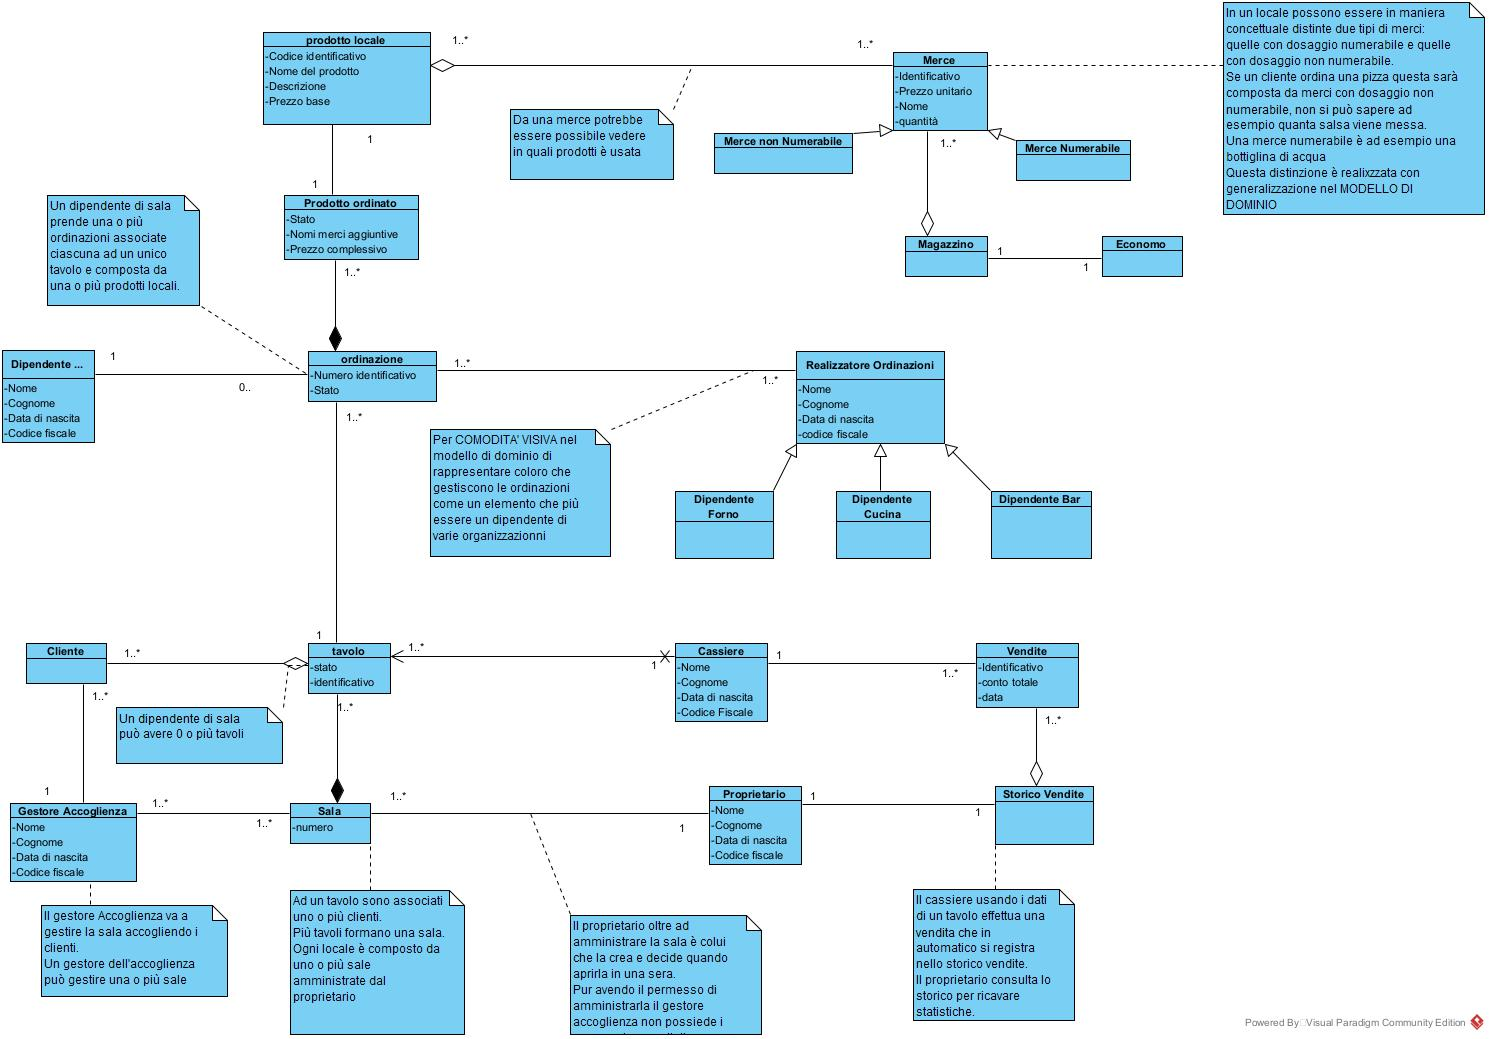
\includegraphics[width=1\textwidth]{Immagini/modello_dominio.jpg}
\end{figure}
Con questo primo diagramma di analisi si sono fatte le prime ipotesi di funzionamento (descritte dai commenti), mettendo in evidenza le relazioni tra le varie entità del sistema.

\begin{enumerate}
	\item In un locale con più camerieri si può verificare la situazione in cui diversi camerieri possono prendere le ordinazioni ad uno stesso tavolo. Con questa ipotesi quindi il cameriere non viene associato direttamente al tavolo, ma all'ordinazione che ha creato per esso.
	\item Il sistema gestisce le merci in modo automatizzato. Esse sono divise in \textit{numerabili} e \textit{non numerabili}. A tal proposito, quando il cameriere crea un'ordinazione che contiene delle merci numerabili, esse vengono immediatamente scalate dal magazzino.
	\item Tutte le vendite completate vengono memorizzate in uno storico.
	\item Il prodotto che viene aggiunto all'ordinazione non equivale al prodotto presente nel menu. Esso infatti può subire delle modifiche come aggiunta o rimozioni di merce dalla sua versione di base. Viene indicato quindi come l'entità \textit{Prodotto Ordinato}.
\end{enumerate}
\newpage
\section{State Chart Diagram}
Alcune entità del sistema hanno delle funzionalità diverse in relazione allo stato in cui si trovano.

\subsection{Tavolo}
\vspace*{0.2cm}
\begin{figure}[H]
	\centering
	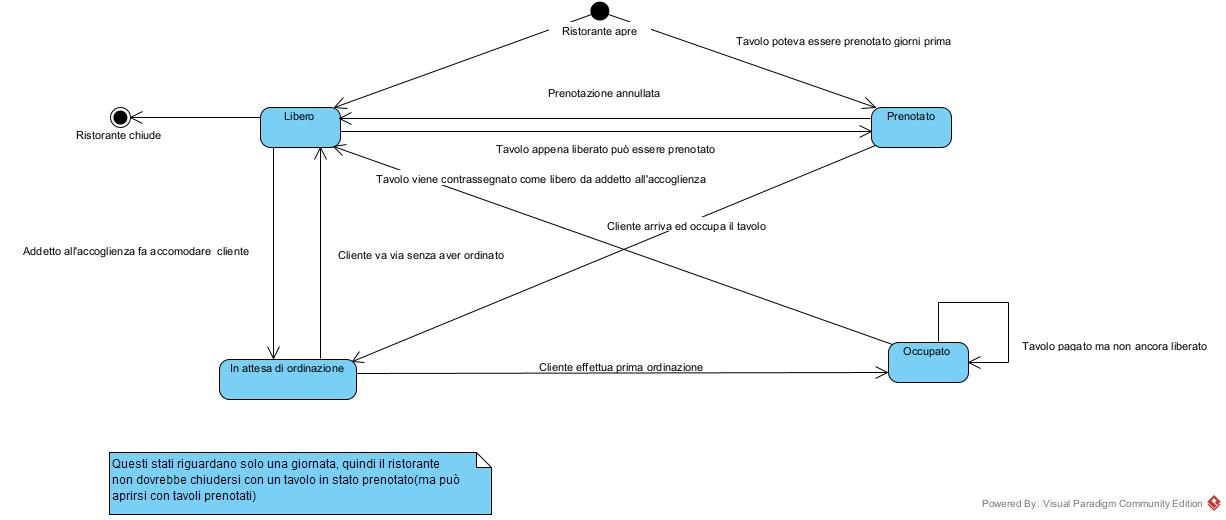
\includegraphics[width=1\textwidth]{Immagini/stati_tavolo.jpg}
\end{figure}
\vspace*{0.1cm}
Questi stati valgono solo durante l'esecuzione del sistema. In teoria il locale non può chiudere con tavoli occupati o in attesa di ordinazione. Attraverso questi stati esiste anche più controllo per evitare errori umani. Ad esempio un cameriere non può prendere le ordinazioni di un tavolo libero, ovvero non occupato da nessun cliente.

\subsection{Prodotto Ordinato}
\vspace*{0.2cm}
\begin{figure}[H]
	\centering
	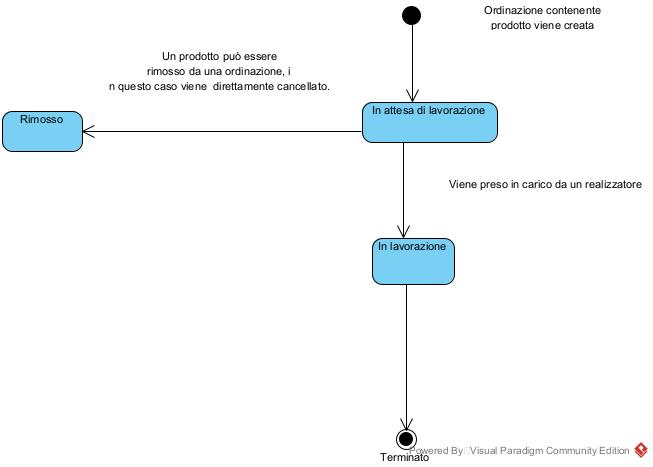
\includegraphics[width=0.8\textwidth]{Immagini/stati_prodotti_ordinati.jpg}
\end{figure}
\vspace*{0.1cm}
Gli stati vengono aggiornati tramite dei feedback di chi realizza i relativi prodotti.

\subsection{Ordine}
\vspace*{0.2cm}
\begin{figure}[H]
	\centering
	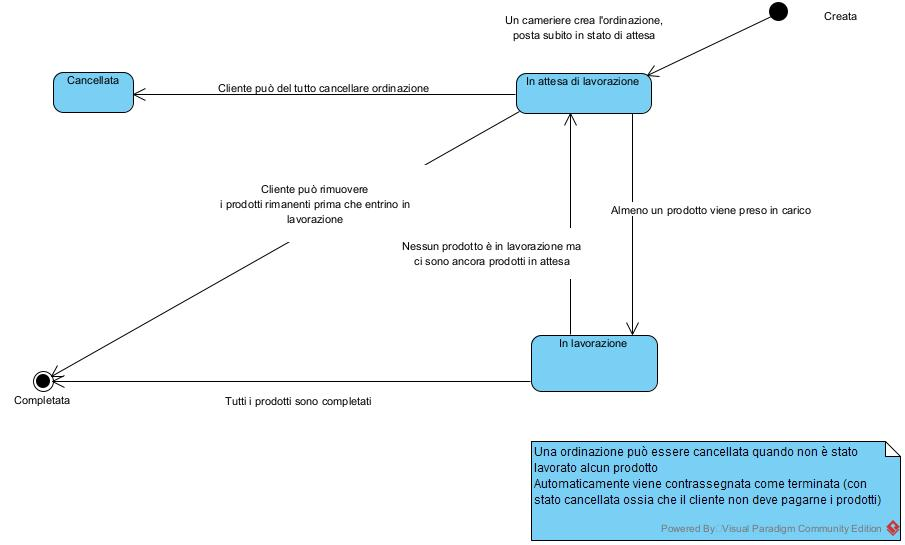
\includegraphics[width=1\textwidth]{Immagini/stati_ordinazione.jpg}
\end{figure}
\vspace*{0.1cm}
Gli stati dell'ordine dipendono molto dagli stati dei prodotti ordinati che lo compongono, essendo infatti un'aggregazione di prodotti.

\newpage
\section{Sequence Diagram di Dominio}
I seguenti sequence diagram sono realizzati solo per indicare le interazioni tra un utente e il sistema.

\subsection{Gestisci Ordinazioni}
\subsubsection{Estensione A}
\begin{figure}[H]
	\centering
	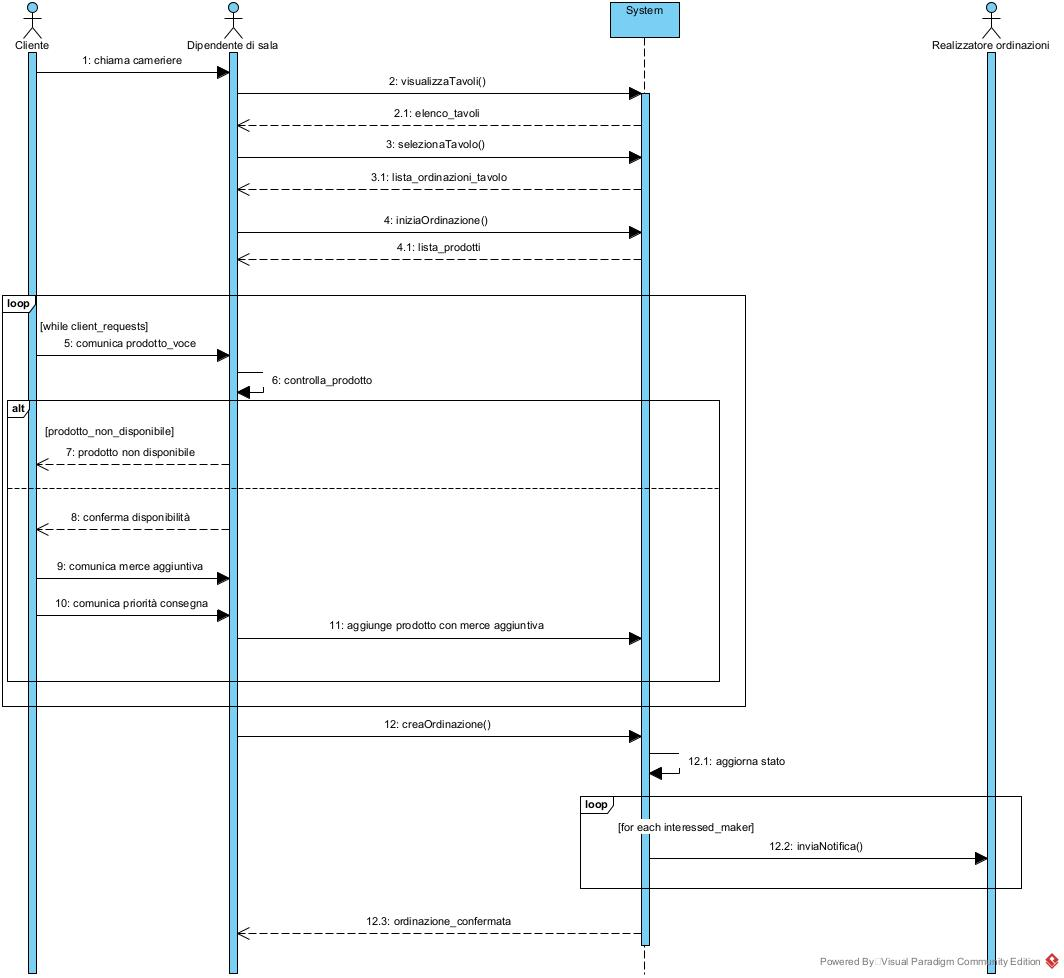
\includegraphics[width=1\textwidth]{Immagini/SSD Gestisci Ordinazioni (Successo).jpg}
\end{figure}

\subsubsection{Estensione B}
\begin{figure}[H]
	\centering
	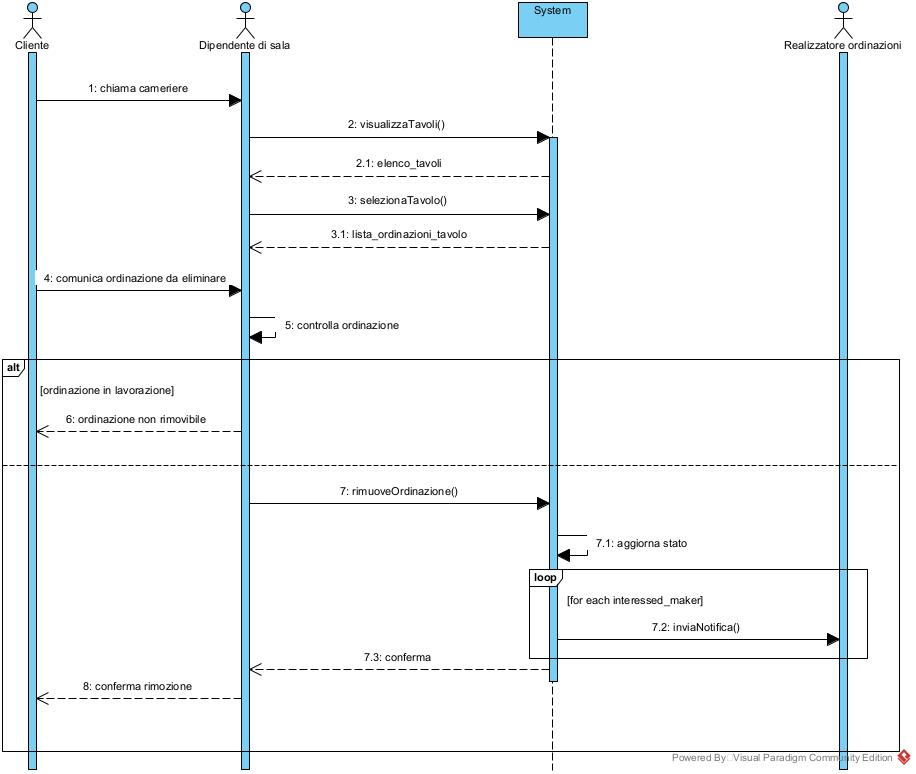
\includegraphics[width=1\textwidth]{Immagini/SSD Gestisci Ordinazione (EstensioneB - Elimina Ordinazione).jpg}
\end{figure}

\subsubsection{Estensione C}
\begin{figure}[H]
	\centering
	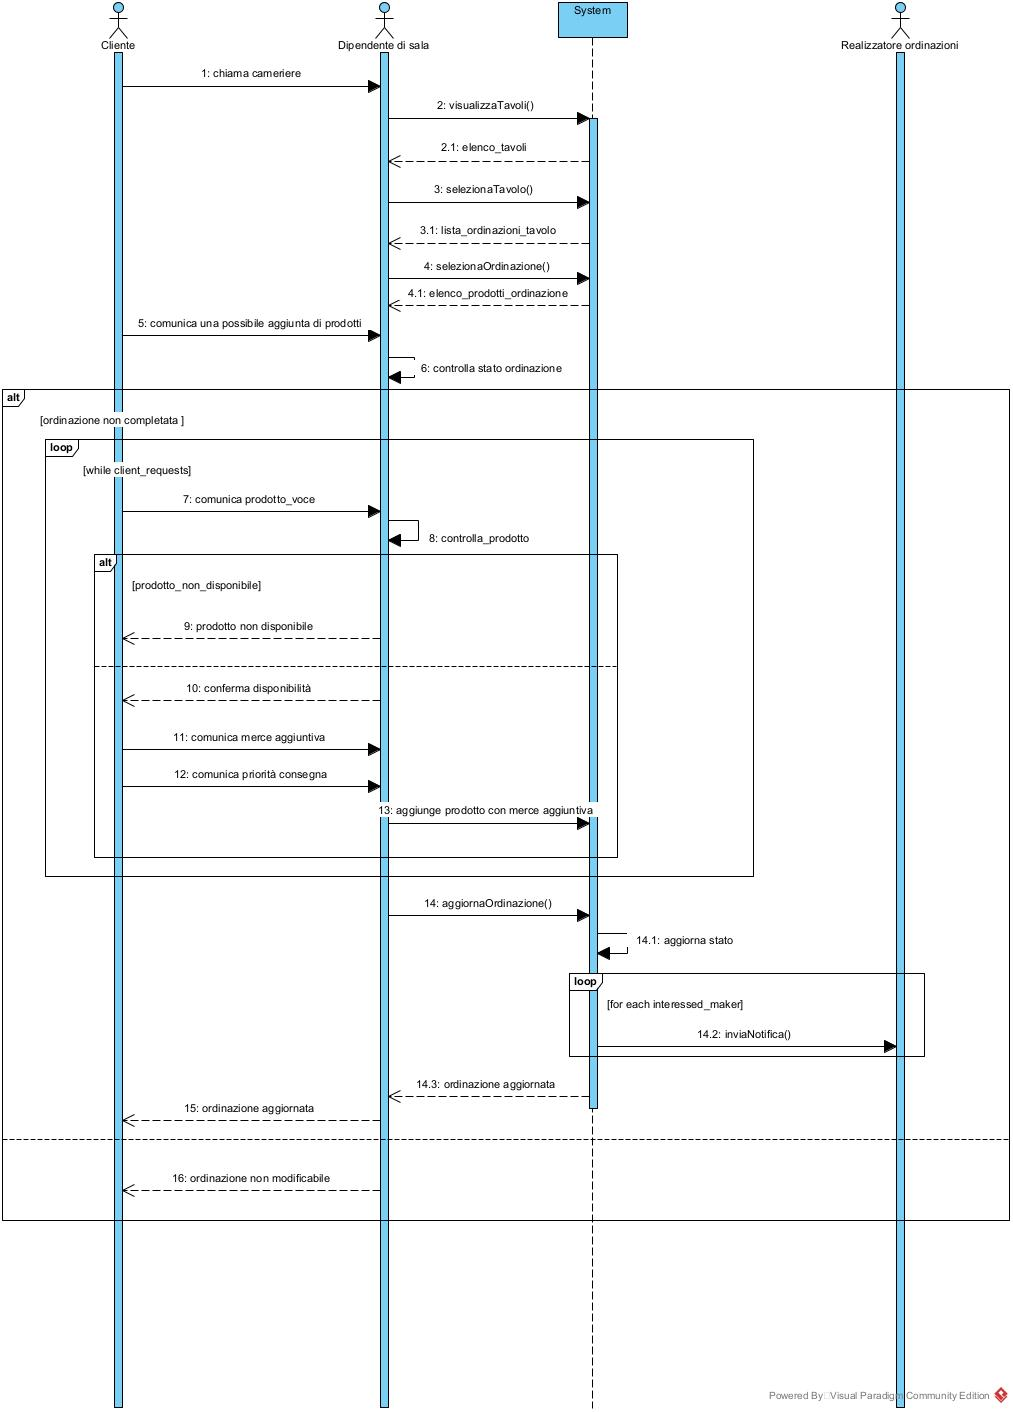
\includegraphics[width=1\textwidth]{Immagini/SSD Gestisci Ordinazione (EstensioneC - Aggiungi prodotto).jpg}
\end{figure}

\subsubsection{Estensione D}
\begin{figure}[H]
	\centering
	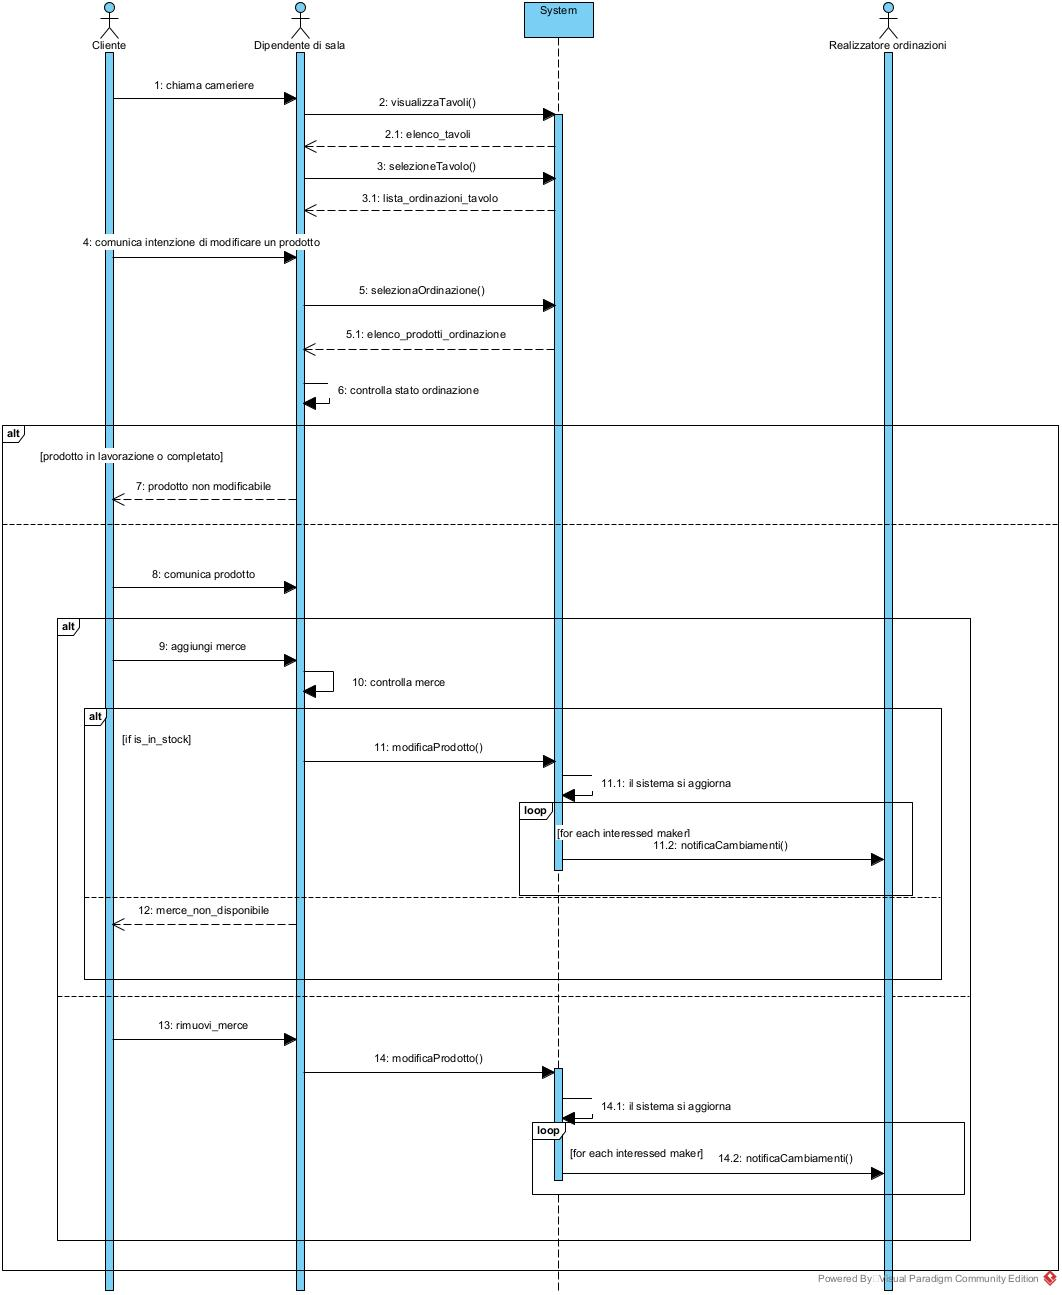
\includegraphics[width=1\textwidth]{Immagini/SSD Gestisci Ordinazione (EstensioneD - Modifica prodotto).jpg}
\end{figure}

\subsubsection{Estensione E}
\begin{figure}[H]
	\centering
	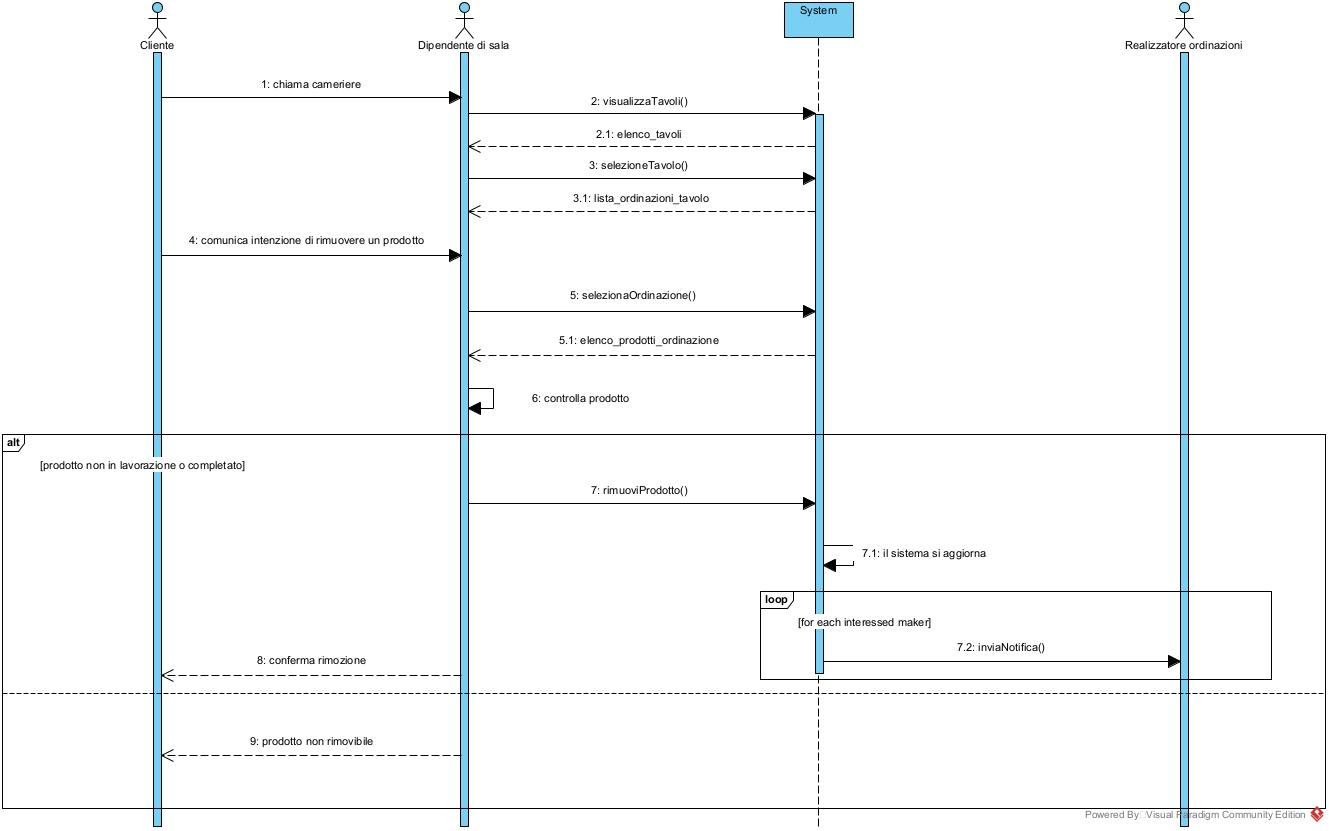
\includegraphics[width=1\textwidth]{Immagini/SSD Gestisci Ordinazioni (Estensione E - Rimuovi prodotto ordinazione).jpg}
\end{figure}

\subsection{Notifica Ordinazione}
\subsubsection{Estensione A}
\begin{figure}[H]
	\centering
	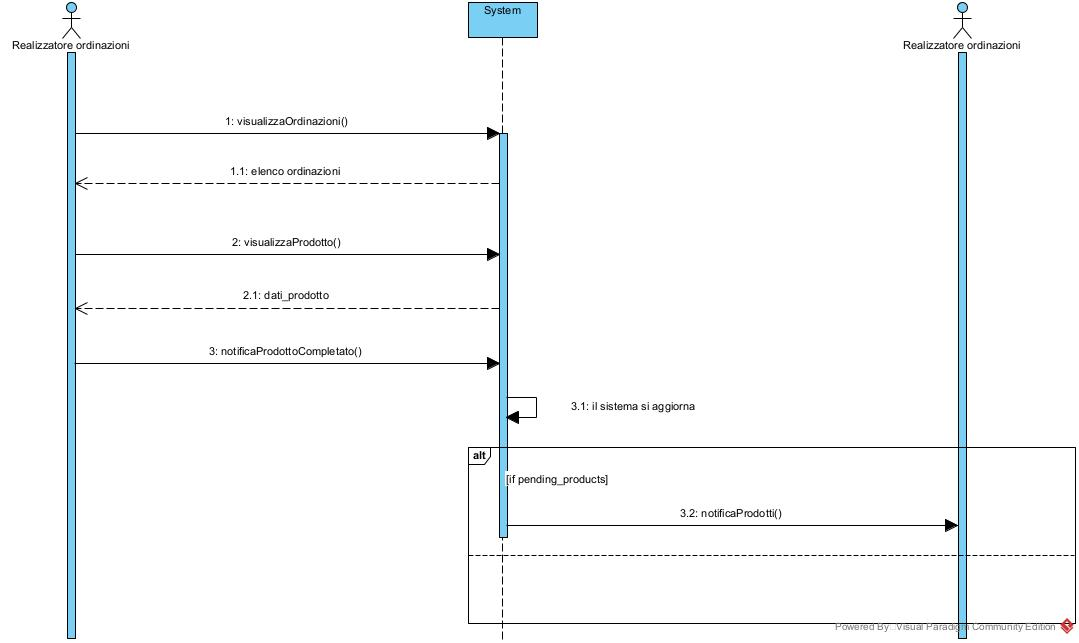
\includegraphics[width=1\textwidth]{Immagini/SSD Notifica Ordinazione.jpg}
\end{figure}

\chapter{Progettazione}
La fase di progettazione prevede principalmente la scelta dell'architettura da usare, su cui costruire il sistema. 
\\Dato il contesto di utilizzo dell'applicativo, la necessità principale è la sincronizzazione del lavoro dei dipendenti. L'obiettivo è quello di informare ogni dipendente del avvenimento di eventi a cui esso è interessato. Ogni azione deve essere memorizzata nel sistema, in conseguenza della quale esso provvede ad avvisare il gruppo di dipendenti relativo.
\\Ad esempio, al momento della registrazione di un'ordinazione da parte di un cameriere, il sistema provvede a notificare lo chef/pizzaiolo (realizzatore in generale) per informalo della nuova pietanza da preparare.
\\Per identificare l'architettura ideale bisogna elencare quali sono i componenti che ne fanno parte e in che modo sono interconnessi.
\begin{itemize}
	\item I componenti sono di due tipologie:
		\begin{itemize}
			\item Dispositivi utente, rappresentano i dispositivi fisici concessi ai dipendenti (smartphone o applicazione desktop)
			\item Sistema centrale, racchiude la logica di gestione e a cui i dispositivi utente possono fare accesso.
		\end{itemize}
	\item I connettori sono principalmente protocolli di rete, in quanto il sistema è pensato anche per dipendenti che hanno la possibilità di spostarsi all'interno del locale e accedere al sistema centrale in modalità remota.
\end{itemize}
Alla base di ciò i componenti devono ricevere dei cambiamenti del sistema tramite opportune \textit{notifiche}, evitando quindi attese attive.

\section{Architettura}
Sulla base delle necessità descritte in precedenza, si è scelto di utilizzare uno stile architetturale del tipo \textbf{Publish-Subscribe}. Per la realizzazione dell'applicativo infatti vengono ripresi tutti i vantaggi dello stile a \textit{invocazione implicita}:
\begin{itemize}
	\item \textit{Disaccoppiamento spaziale}: tutti i componenti sono altamente disaccoppiati, favorendo la scalabilità del sistema. Il proprietario può quindi assumere un numero di dipendenti variabile senza conseguenze.
	\item \textit{Disaccoppiamento di sincronizzazione}: tutti i componenti non lavorano in "polling", ovvero in attese attive che possono bloccare il sistema.
	\item \textit{Disaccoppiamento temporale}: tutti i componenti possono essere volatili nel sistema.
\end{itemize}
In relazione ai componenti descritti, tutti i dipendenti sono dei \textit{Subscribers} mentre il sistema centrale è l'unico \textit{Publisher}.
\\I dipendenti, effettuando l'accesso, si iscrivono in automatico al Publisher.
Dato che il sistema può contenere un numero notevole di dipendenti, il Publisher fa uso di \textbf{Proxy} per smistare i messaggi solamente a specifici Subscribers.
\\Essi infatti all'atto del login non conoscono i Proxy del sistema, ma è il sistema stesso che li racchiude in gruppi (con lo stesso ruolo) e li associa a determinati Proxy. Tutto ciò si traduce in una distribuzione più efficiente del calcolo computazionale.
\\Riassumendo quindi:
\begin{table}[H]
	\centering
	\begin{tabular}{|l | p{0.75\linewidth} |}
		\hline
		\textbf{Componenti} & Publisher, Subscribers, 
		Proxy \\
		\hline
		\textbf{Connettori} & Protocolli di rete \\
		\hline
		\textbf{Dati} & Notifiche, Richieste di informazioni, Informazioni pubblicate \\
		\hline
		\textbf{Topologia} & Subscribers sono connessi al Publisher indirettamente, ricevendo e inviando notifiche attraverso i Proxy \\
		\hline
		\textbf{Vantaggi} & Subscribers sono tutti disaccoppiati lavorando in parallelo. Le notifiche vengono ben distribuite grazie ai Proxy \\
		\hline
		\textbf{Svantaggi} & Il controllo computazionale è caricato tutto sul sistema centrale. Nessuna conoscenza di quali componenti risponderanno ad un eventi \\
		\hline
	\end{tabular}
\end{table}


\subsection{Component Diagram}
\begin{figure}[H]
	\centering
	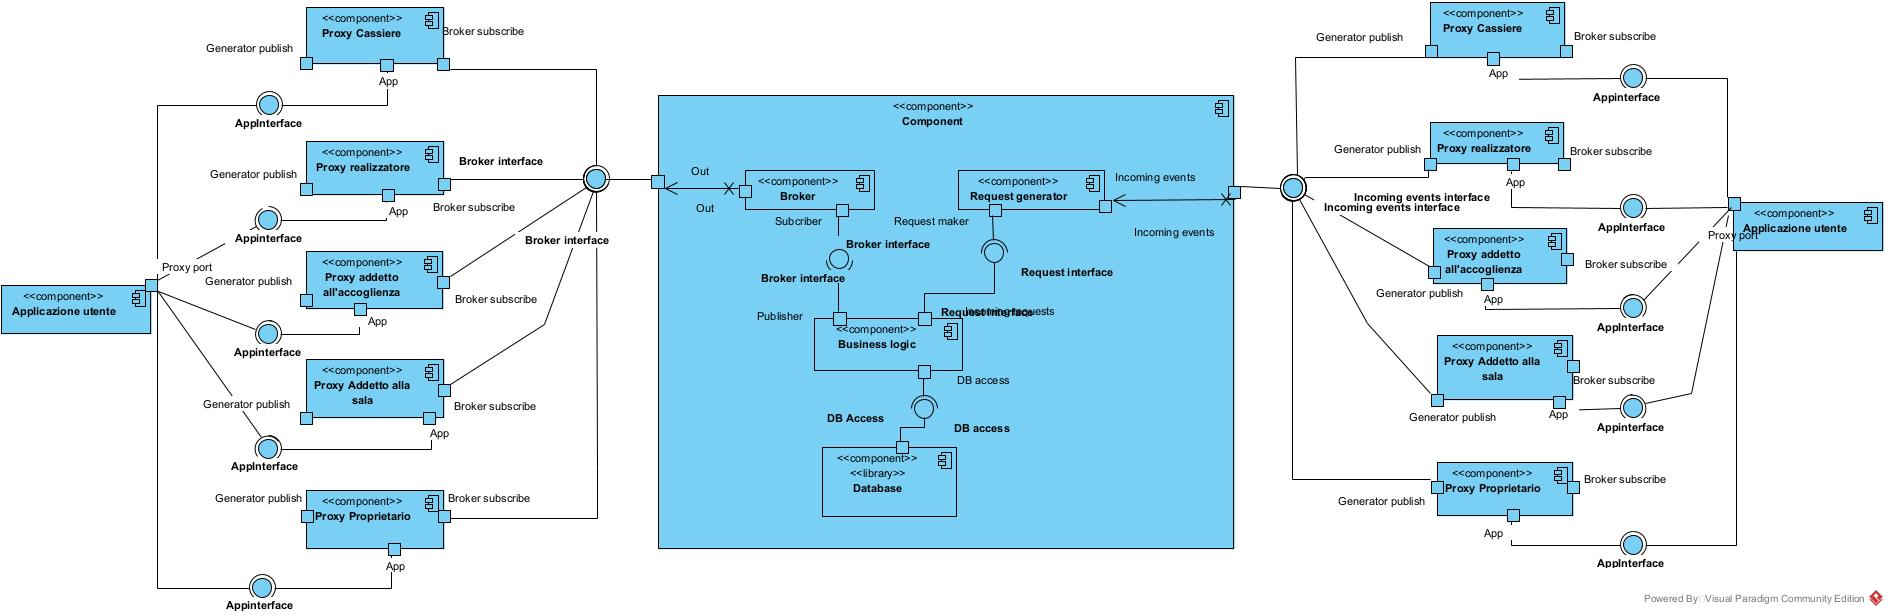
\includegraphics[width=1\textwidth]{Immagini/dynamic components.jpg}
\end{figure}

\section{Database}
Il database deve contenere le informazioni di base che devono essere utilizzate, a partire dai dipendenti che vengono registrati nel sistema e finire con le ordinazioni che vengono effettuate durante l'utilizzo del sistema.
\begin{figure}[H]
	\centering
	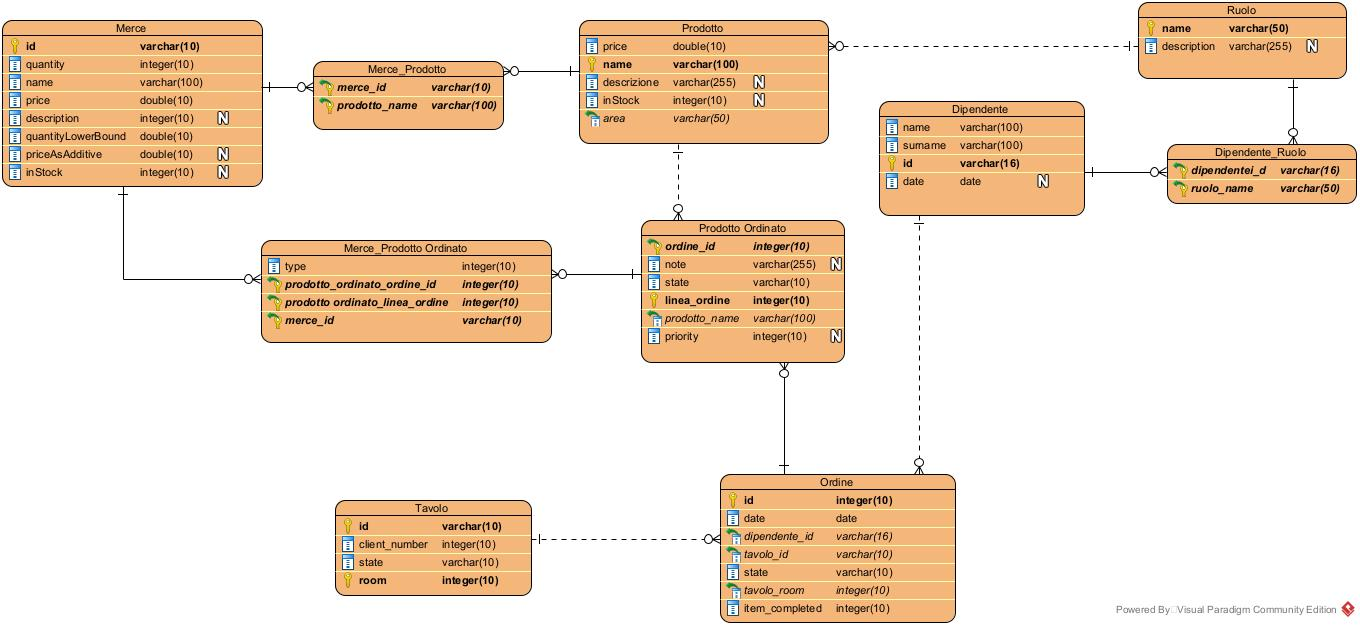
\includegraphics[width=1\textwidth]{Immagini/database.jpg}
\end{figure}
Le caratteristiche principali del database sono le seguenti:
\begin{enumerate}
	\item Le merci hanno, oltre alle informazioni di base quali prezzo, codice identificativo, nome, etc, hanno un attributo \textit{priceAsAdditive}. Tale attributo, se non nullo, indica il prezzo da aggiungere se quella merce è usata come merce aggiuntiva di un prodotto.
	\item Il \textit{Prodotto Ordinato} è un'associazione ternaria tra \textit{Ordine}, \textit{Prodotto} e \textit{Merce}.
	 \item Ogni prodotto ha un attributo collegato all'entità \textit{Ruoli}. Esso serve per indicare a che attività appartiene quel prodotto.
\end{enumerate}
Il precedente database si riferisce solo ai casi d'uso che si sono scelti di implementare. Non contiene, ad esempio, la gestione delle vendite e lo storico del locale.

\section{Deployment Diagram}
\section{Class Diagram}
\section{Sequence Diagram}
\chapter{Implementazione}
La parte implementativa riguarda il processo di implementazione, le tecniche e i framework utilizzati durante lo sviluppo sia del Main System e del database backend, sia dell'infrastruttura di comunicazione dei Proxy e sia dell'interfaccia client dell'applicazione Android. 

\section{Database}
Per le nostre esigenze, vi era la necessità di una base di dati sviluppabile in breve tempo e con un DBMS documentato e facile col quale comunicare. Sulla base di scelte implementative fatte anche nel Main System, la scelta è ricaduta su \textbf{PostgreSQL}. 
\\PostgreSQL è un database relazionale, la cui progettazione è stata semplificata grazie alle conoscenze preliminari acquisite in altri corsi. Implementativamente è stato definito uno \textit{schema} che racchiude tutte le tabelle necessarie per la memorizzazione dei dati, chiamato \textit{Restaurant}. Inoltre il modello relazionale non è del tutto identico al modello degli oggetti del Main System; questo però non provoca problemi di implementazione data la natura ben chiara delle informazioni.
\vspace{0.5cm}
\\All'interno del package \textit{DataAccess} della Business Logic del Main System sono state definite tutte le query per prelevare le informazioni dalla base di dati. In tal modo l'accesso al database è del tutto mascherato e controllato. Ogni elemento del package \textit{Areas} può accedere solo a determinate aree del database, mascherando tutti i dati memorizzati. Ad esempio l'area utente può accedere solo ad informazioni relative agli utenti, e non quelle relative al menù o alle merci a disposizione.

\section{Main System}
Il Main System è il cuore dell'applicazione, in quanto ne è il cervello pensante. L'implementazione di questa parte conta diverse centinaia di linee di codice, poiché gestisce tutte le meccaniche di creazione, eliminazione e aggiornamento di un evento relativo a tutti i possibili ruoli. Lo sviluppo, in concomitanza con i test, ha richiesto un'analisi attenta e precisa della modularità del codice. 
\\In particolare, la scelta di un framework da utilizzare si è rivelata fondamentale per gestire opportunamento lo sviluppo. La scelta è ricaduta sul framework \textbf{Spring Boot} versione 2.5.5, versione di Java 11 e Maven per la gestione delle dipendenze. Tale decisione è dovuta alle meccaniche di injection fornite da Spring, che hanno reso estremamente semplice e scalabile la comunicazione con PostgreSQL. 
\\Spring fornisce infatti diverse annotazioni estremamente veloci ed efficaci quali @Autowire per effettuare la dependency injection di oggetti che possono essere servizi, controller o semplici bean di configurazione. Ciò ha reso non solo di più semplice lettura il codice, ma ci ha anche notevolmente risparmiato il tempo di dover implementare le meccaniche di comunicazione fra classi sia interne sia esterne ai package implementati. \vspace{0.5cm}
\\Il Main System utilizza queste facilitazioni definendosi di base la logica di controllo e poi un intreccio di controller organizzati gerarchicamente: un usersController, un restaurantController ed un menuAndWareHouseController, tutti organizzati sotto un unico GeneralController, esteso dal SystemController che ha il compito di interfacciare il sistema con il \textbf{Request Generator} e con il \textbf{Broker}. Ogni controller di base si occupa poi della comunicazione col database per le informazioni di proprio interesse, scambiandole con l'esterno attraverso il System Controller.

\subsection{Request Generator}
Il Request Generator è il componente che si interfaccia coi proxy adibiti alla ricezione di richieste da parte dell'applicazione. 
\\L'interfaccia sviluppata di basa su due componenti principali: 
\begin{itemize}
	\item Il \textbf{JMS}, versione 2.0;
	\item \textbf{ActiveMQ Artemis}, un MOM configurabile in maniera particolarmente rapida: basta usare un comando per dichiararsi un broker ed un altro per avviarlo e subito si può iniziare a sperimentare.
\end{itemize}
I messaggi scambiati sono tutti in formato JSON. La progettazione rende di fatto già scalabile la comunicazione, di conseguenza il Request Generator ha il solo compito di fornire l'interfaccia verso Artemis attraverso un controller che prenda in carico, attraverso il JMS, i messaggi che sulle diverse code vengono prodotti. \vspace{0.5cm}
\\Anche per il Request Generator è stato usato Spring Boot. In particolare, di fondamentale importanza è stata la dependency \textit{Spring for Apache ActiveMQ 5}. Essa mette a disposizione l'infrastruttura necessaria alla comunicazione coi server Artemis utilizzabile attraverso l'interfaccia, da estendere, MessageListener. E' per questo motivo che Request Generator implementa diversi controller a seconda della coda di messaggi: ogni controller modifica il metodo onMessage() per gestire opportunamente il messaggio JSON, la cui struttura può cambiare a seconda della coda sul quale si trova, che riceve. Internamente, il dispatcher si preoccupa poi solo di reindirizzare opportunamente al Main System i messaggi che arrivano implementando i controller del Request Generator e il System Controller e gestendone le chiamate a funzione.  

\subsection{Broker}
Il Broker ha il compito esattamente opposto al Request Generator: smistare i messaggi sulle code in maniera tale da informare l'applicazione utente degli eventi ai quale essa è interessata. 
La struttura, poiché ricettiva, riceve i messaggi da pubblicare attraverso il System Controller che implementa un'interfaccia, la BrokerInterface, che poi il Dispatcher estende. \vspace{0.5cm}
\\Anche il Broker utilizza il JMS e ActiveMQ Artemis per comunicare con l'applicazione attraverso i proxy. La differenza principale col Request Generator è che il Broker ha bisogno di aprire il messaggio JSON inviato dall'applicazione per smistarlo correttamente sulla base del codice nominativo dell'area, di fatto codice univoco per la coda su cui smistare.
\\Come il Request Generator, non effettua poi alcuna modifica sui messaggi, preoccupandosi soltanto di gestirne il corretto invio. La comunicazione col Main System avviene anche qui attraverso semplice chiamata a funzione. 

\section{Proxy}
I proxy sono l'impalcatura su cui si fonda la rete di messaggi tra applicazione e sistema. 
\\L'idea di implementare dei proxy è nata dalla difficoltà che l'applicazione aveva nel comunicare con il sistema in maniera corretta, gestendo correttamente tutti i tipi di messaggi, che nel concreto sono tutti eventi di diversa natura, che bisognava inviare e ricevere. 
\\Da ciò, l'idea dei proxy per rendere non solo più semplice la comunicazione, affibiando a loro il compito di incaricarsi della comunicazione, ma anche per fornire un'interfaccia più scalabile e flessibile ad eventuali modifiche e aggiornamenti. \vspace{0.5cm}
\\Anche l'implementazione dei proxy è basata su Spring Boot. Le dependency utilizzate sono \textbf{Spring Web} e \textbf{Spring for Apache ActiveMQ Artemis}. 
\\I proxy hanno infatti sia il compito di fungere da client per il Request Generator sia quello di fungere da server per il Broker. Di conseguenza, la prima dependency di Spring mette a disposizione l'infrastruttura generale per aprire un server Tomcat in ascolto in localhost di default sul porto 8080, configurazione che può essere modificata attraverso il file di proprietà.
\\Vi sono diversi proxy, ma tutti in generale hanno la stessa struttura ed implementazione che differisce solo sulla base dei messaggi che devono leggere e scambiare. \vspace{0.5cm}
\\Per la gestione dei messaggi HTTP, i proxy utilizzano dei controller specifici che si preoccupano di istanziare un metodo wrapper per le POST effettuate al filepath indicato. La sintassi è la seguente:

\begin{itemize}
	\item @PostMapping(valude= {filepath})
\end{itemize}

Attraverso quest'annotazione, è possibile gestire in ricezione le richieste POST che arrivano dall'applicazione al filepath indicato. In questo modo, ogni proxy deve solo preoccuparsi, in ricezione, di girare poi il messaggio sulla coda corretta, attraverso una convertAndSend, cioè un metodo della classe JmsTemplate fornita da Spring nella libreria \textit{org.springframework.jms.core.JmsTemplate}. \vspace{0.5cm}
\\In fase di ricezione, come per il Request Generator, ogni proxy deve invece mettersi in ascolto sui messaggi delle codce che il Broker riempie. Il lavoro che in questo caso il proxy deve effettuare è più delicato: 

\begin{enumerate}
      \item Deve spacchettare il messaggio JSON per comprendere di che tipo di evento si tratti;
            
      \item Se si tratta di un messaggio di registrazione, deve registrare l'uri dell'applicazione al proprio Webhook e rispedire il messaggio al destinatario corretto specificando il proprio uri di destinazione;
      
      \item Se si tratta di un messaggio da spedire ad un'applicazione, suppone che quest'ultima già conosca il proprio uri di destinazione e si preoccupa solo di verificare che essa sia registrata al proprio Webhook;
      \begin{itemize}
        \item In tal caso, manda in broadcast se più applicazioni sono interessate altrimenti manda al singolo destinatario interessato. 
      \end{itemize}
      
      \item Impacchetta il messaggio nuovamente in un JSON ed invia. 
\end{enumerate}

L'invio è gestito sempre attraverso richieste POST all'indirizzo contenuto nella lista Webhook attraverso funzioni di utilità che fanno utilizzo della libreria Spring \textit{org.springframework.web.client.RestTemplate}. 

\chapter{Test}


\end{document}
